\documentclass[conference]{IEEEtran}
\IEEEoverridecommandlockouts

\usepackage{cite}
\usepackage{amsmath,amssymb,amsfonts}
\usepackage{graphicx}
\usepackage{textcomp}
\usepackage{xcolor}
\usepackage{booktabs}
\usepackage{url}
\usepackage{hyperref}

\graphicspath{{../results/figures/}{../results/breast_cancer/figures/}}

% Single source of truth: report_numbers.py writes paper/numbers.tex from the
% aggregate results. Input it directly so the IEEE paper never drifts from the
% canonical macros (and from the NeurIPS-format paper that shares them).
% Auto-generated by scripts/report_numbers.py -- do not edit by hand.
\newcommand{\Nspecs}{16}
\newcommand{\Nspots}{2688}
\newcommand{\Ngenes}{18078}
\newcommand{\ClustMin}{8}
\newcommand{\ClustMax}{22}
\newcommand{\ClustMean}{13.2}
\newcommand{\ClustStd}{3.9}
\newcommand{\SpotSthreeMean}{0.80}
\newcommand{\SpotStableFrac}{57\%}
\newcommand{\SpotFragileFrac}{4\%}
\newcommand{\GeneRobustFrac}{28\%}
\newcommand{\GeneFragileFrac}{69\%}
\newcommand{\AriMean}{0.68}
\newcommand{\AriMin}{0.49}
\newcommand{\AriMax}{0.90}


\def\BibTeX{{\rm B\kern-.05em{\sc i\kern-.025em b}\kern-.08em
    T\kern-.1667em\lower.7ex\hbox{E}\kern-.125emX}}

\begin{document}

\title{MOSAIC: Measuring How Analysis Choices\\
Change Results in Spatial Transcriptomics}

\author{
\IEEEauthorblockN{
Sparsh Roy\IEEEauthorrefmark{1},
Adharv Pemmasani\IEEEauthorrefmark{2},
Kevin Zhou\IEEEauthorrefmark{2},
Arhaan Shah\IEEEauthorrefmark{3},
Vihaan Joshi-Apte\IEEEauthorrefmark{3}\\
Samuel Girmachew\IEEEauthorrefmark{2},
William Langille\IEEEauthorrefmark{2}}
\IEEEauthorblockA{
\IEEEauthorrefmark{1}Massachusetts Institute of Technology, sparshr@mit.edu\\
\IEEEauthorrefmark{2}Hopewell Valley Central High School\\
\IEEEauthorrefmark{3}Paradise Valley High School}
}

\maketitle

\begin{abstract}
Analyzing spatial transcriptomics data involves many choices that are each
reasonable but somewhat arbitrary: normalization, feature selection,
dimensionality reduction, neighborhood graph, clustering algorithm and
resolution, and the test used to call spatially variable genes. MOSAIC runs
\Nspecs{} such pipelines on the same tissue section and measures how much
the results agree using a \emph{Spatial Stability Score} ($S^3$), computed
per spot, per gene, and for summary statistics. Cluster labels are matched
across pipelines with the Hungarian algorithm. On two mouse-brain sections,
the number of spatial domains ranges from \ClustMin{} to \ClustMax{}
depending on the pipeline (mean pairwise Adjusted Rand Index \AriMean{}).
A Type-II ANOVA attributes \VarTopFrac{} of the variation in domain count
to clustering \VarTopAxis{}. Low-stability spots cluster at domain
boundaries (gap \StakesGap{}, $p\,\StakesP{}$), and stability is not
correlated with sequencing depth ($r=\ConfoundR{}$). On a human
breast-cancer section with pathology annotations, stability is lowest in
the region annotated as surrounding tumor, and this holds under bootstrap
resampling and a depth-stratified permutation test. We also find that
combining all pipelines into a co-association consensus recovers reference
anatomy about as well as the best single pipeline (ARI \ConsensusARI{};
better than the median pipeline in \ConsensusBeatsMedianPct{} of settings),
without needing the reference labels to choose a pipeline, and that per-spot
$S^3$ predicts where the consensus is wrong (AUC \ConsensusUncAUC{}).
Finally, a classifier trained on features from a single pipeline predicts
which spots will be unstable across all pipelines (AUC \FragPredAUC{} with
random splits, lower with spatially blocked splits). Code, configuration,
and figure scripts are public.
\end{abstract}

\begin{IEEEkeywords}
spatial transcriptomics, computational pathology, multiverse analysis,
specification-curve analysis, reproducibility, ensemble clustering,
uncertainty quantification
\end{IEEEkeywords}

\section{Introduction}
\label{sec:intro}

There is rarely one correct way to analyze a spatial transcriptomics
dataset. Going from raw counts to a map of spatial domains requires
choosing a normalization, a number of highly variable genes (HVGs), a number
of principal components, a neighbor graph, Leiden~\cite{traag2019louvain} or
Louvain~\cite{blondel2008fast} clustering and a resolution, and a test for
spatially variable genes (SVGs)~\cite{moran1950notes,
svensson2018spatialde, weber2023nnsvg}. Each option has been used in
published work, so each is defensible. But a study usually runs one
pipeline and reports its output.

Gelman and Loken call this the \emph{garden of forking
paths}~\cite{gelman2013garden}: even without deliberate cherry-picking, a
reported result can depend on which path was taken rather than on the
biology. \emph{Multiverse analysis}~\cite{steegen2016increasing} addresses
this by running many reasonable analyses and reporting the spread of
outcomes. When 70 teams analyzed the same neuroimaging dataset, they
reached substantially different conclusions~\cite{botvinik2020variability}.
Spatial transcriptomics benchmarks usually compare methods against a
reference; here we instead ask how much reasonable analysis choices change
the results on a fixed tissue section.

This paper is a descriptive pipeline-sensitivity (multiverse) analysis of
three public Visium sections. We contribute:

\begin{enumerate}
\item[\textbf{C1}] A configurable pipeline and a simple agreement score
  ($S^3$) computed per spot, per gene, and for summary statistics
  (\S\ref{sec:method}).
\item[\textbf{C2}] Descriptive measurements of how much spatial domains,
  SVG calls, and a downstream classifier change across pipelines on two
  mouse-brain sections and one breast-cancer section (\S\ref{sec:results},
  \S\ref{sec:tumor}), with a full 864-pipeline factorial on two of the
  sections (\S\ref{sec:factorial}).
\item[\textbf{C3}] Two exploratory uses of the pipeline collection: a
  co-association consensus and a single-pipeline predictor of low-agreement
  spots (\S\ref{sec:consensus}, \S\ref{sec:downstream}).
\end{enumerate}

\section{Related Work}
\label{sec:related}

\textbf{Multiverse analysis.}
Steegen~\emph{et al.}~\cite{steegen2016increasing} introduced multiverse
analysis and Simonsohn~\emph{et al.}~\cite{simonsohn2020specification}
specification curves, both in psychology. Gelman and
Loken~\cite{gelman2013garden} explained why analytic flexibility is a
problem even without deliberate $p$-hacking, and
Botvinik-Nezer~\emph{et al.}~\cite{botvinik2020variability} showed its
effect across 70 fMRI analysis teams. Spatial omics adds the problem that
cluster labels are arbitrary and must be matched before they can be
compared.

\textbf{Spatial transcriptomics pipelines.} Standard analyses use
SCANPY~\cite{wolf2018scanpy} and Squidpy~\cite{palla2022squidpy}, with
Louvain~\cite{blondel2008fast} or
Leiden~\cite{traag2019louvain,traag2011narrow} clustering and SVG detection
by Moran's $I$~\cite{moran1950notes},
SpatialDE~\cite{svensson2018spatialde}, or nnSVG~\cite{weber2023nnsvg}.
Reference atlases such as the DLPFC dataset~\cite{maynard2021transcriptome}
are used for benchmarking, and reviews~\cite{luecken2019current} compare
methods against such references. Multi-platform integration tools such as
MOSAIK~\cite{baptista2025mosaik} combine data sources but do not measure
analytical sensitivity.

\textbf{Consensus clustering.} Our co-association consensus
(\S\ref{sec:consensus}) follows classical consensus
clustering~\cite{monti2003consensus} and cluster
ensembles~\cite{strehl2002cluster}, which usually combine partitions from
one method under resampling or different random initializations. We
combine partitions from pipelines that differ in normalization, features,
graph, and clustering. We have not compared it against other ensemble
methods.

\textbf{Concurrent work on per-spot instability.} Wu
\emph{et al.}~\cite{wu2026instability} independently developed InSTability,
which measures per-spot disagreement across seven clustering methods
(BayesSpace, GraphST, Leiden, Louvain, SEDR, STAGATE, SpiceMix) on 18
benchmark samples, focusing on variation from repeated runs and choice of
method. We vary earlier preprocessing steps as well. We have not compared
the two measures directly.

\textbf{Related work in other domains.} Similar pipeline dependence appears
elsewhere. Zhou and Roy~\cite{zhou2026matched} find that for EEG foundation
models on motor imagery, which architecture performs better depends on the
input pipeline. Roy \emph{et al.}~\cite{roy2026kaisen} find that the effect
of a fairness mitigation step in clinical risk models varies more across
cohort samples than across diseases, and recommend reporting the spread
across runs.

\section{Method}
\label{sec:method}

\subsection{Pipeline space}
Each analysis stage is an axis (Table~\ref{tab:space}); the full Cartesian
product has 864 combinations. Most results use a curated set of \Nspecs{}
pipelines built around one canonical pipeline (log1p, 3000 Seurat HVGs, 30
PCs, $k=15$, Leiden at resolution 0.5): 12 change one setting from it, 10
change two, and 7 change three or more. The SVG test is fixed at Moran's
$I$. Because the curated set is not a factorial design and its axes are
correlated, it describes sensitivity around one pipeline rather than across
the whole space. Section~\ref{sec:factorial} reports the full factorial on
two sections.

\begin{table}[t]
  \centering
  \caption{The analytical pipeline space.}
  \label{tab:space}
  \footnotesize
  \setlength{\tabcolsep}{4pt}
  \begin{tabular}{@{}p{0.30\columnwidth}p{0.63\columnwidth}@{}}
    \toprule
    Stage & Options \\
    \midrule
    Normalization & total-count to $10^4$, then $\log(1+x)$, $\sqrt{x}$, or no transform \\
    Feature selection & Seurat or Cell Ranger HVG flavor; \{2000, 3000, 5000\} genes \\
    Dimensionality & PCA, \{30, 50\} components \\
    Neighbor graph & $k$-NN in PCA space, $k \in \{6, 10, 15\}$ \\
    Clustering & Leiden / Louvain; resolution $\in \{0.3,0.5,0.8,1.2\}$ \\
    SVG test & Moran's $I$, BH-FDR $<0.05$ (fixed) \\
    \bottomrule
  \end{tabular}
\end{table}

\subsection{Pipeline details}
Each specification starts from the stored raw counts. Normalization scales
each spot to $10^4$ total counts (\texttt{sc.pp.normalize\_total}) and then
applies $\log(1+x)$, $\sqrt{x}$, or nothing. HVGs are selected with
\texttt{sc.pp.highly\_variable\_genes} using the \texttt{seurat} or
\texttt{cell\_ranger} flavor. The neighbor graph is SCANPY's default
\texttt{sc.pp.neighbors} on the PCA embedding (UMAP-style connectivities,
Euclidean distance); it is built in expression space, not physical space,
so clustering is not spatially constrained. Leiden uses the
\texttt{leidenalg} backend and Louvain uses igraph's multilevel method,
both at the given resolution. Moran's $I$ uses
\texttt{sq.gr.spatial\_autocorr} on Squidpy's default Visium grid graph
(\texttt{sq.gr.spatial\_neighbors}) with 100 permutations and BH
correction over all HVGs tested in that specification. All random steps
use seed 42. Repeated runs of a fixed specification with the same
software versions gave identical spot labels; we have not checked
determinism across library versions. Package versions are pinned in the
repository (\texttt{constraints.txt}).

\subsection{Agreement score}
\label{sec:s3}
Let $\mathcal{S}$ be the set of specifications, $N=|\mathcal{S}|$, and
$c_s(i)\in\{1,\dots,K_s\}$ the cluster label of spot $i$ under $s$. Cluster
labels are arbitrary, so we match each specification to a reference
specification $s_0$ (the canonical pipeline) using the overlap matrix
$M^{(s)}_{ab}=|\{i: c_{s_0}(i)=a \wedge c_s(i)=b\}|$ and the one-to-one
assignment that maximizes total overlap (Hungarian
algorithm~\cite{kuhn1955hungarian}). If $s$ has more clusters than $s_0$,
the unmatched clusters all receive one shared overflow label, which is the
same in every specification. If $s$ has fewer clusters, some reference
labels go unused. With matched labels $\tilde c_s(i)$, per-spot agreement
is the fraction of specifications that give the most common label,
\begin{equation}
  S^3_{\text{spot}}(i) = \frac{1}{N}\max_{\ell}\left|\{s\in\mathcal{S}:\tilde
  c_s(i)=\ell\}\right| \in \left[\tfrac1N,1\right].
\end{equation}
Per-gene agreement is the fraction of specifications that call gene $g$ a
significant SVG,
\begin{equation}
  S^3_{\text{gene}}(g) = \frac1N\sum_{s\in\mathcal{S}} \mathbb{1}[g\in\text{SVG}_s].
  \label{eq:s3gene}
\end{equation}
For summary statistics such as the number of domains, we report the mean,
standard deviation, and range across $\mathcal{S}$. We also report mean
pairwise Adjusted Rand Index (ARI)~\cite{hubert1985comparing} between
specifications, which needs no label matching.

\textbf{Limitations of $S^3_{\text{spot}}$.} One-to-one matching handles
splits and merges poorly: when one pipeline splits a reference cluster in
two, only one half can match, and the shared overflow label can make spots
in unrelated unmatched clusters look like they agree. $S^3_{\text{spot}}$
also depends on the reference. Recomputing it with each of the
\RefRobustN{} mouse-brain specifications as the reference, the
section-wide mean stays in $[\RefRobustAggMeanRange{}]$ (standard
deviation \RefRobustAggMeanStd{}), but per-spot maps from different
references correlate at only \RefRobustMeanPearson{} on average (lowest
pair \RefRobustMinPearson{}), and a spot's score varies by
\RefRobustMeanPerSpotStd{} (standard deviation) across references. The
score is therefore not a reference-independent measure of spot stability.
We report it mainly as section-wide and regional summaries, and treat
per-spot uses (\S\ref{sec:consensus}, \S\ref{sec:downstream}) as
exploratory. A label-free local measure based on pairwise co-clustering
would avoid both problems and is left for future work.

\subsection{Statistical procedures}
\label{sec:stats}
We describe these procedures exactly because they have known weaknesses.
\textbf{Permutation tests} keep per-spot scores fixed and shuffle region or
boundary labels among spots ($B{=}1000$, preserving group sizes), with a
one-sided empirical $p$-value using add-one correction. The smallest
attainable value is $1/1001\approx0.001$, which we report as $p=0.001$.
\textbf{Depth-stratified tests} shuffle labels only within
sequencing-depth deciles. Both tests treat spots as exchangeable and break
the spatial arrangement of the tissue, so they ignore spatial
autocorrelation and their $p$-values are likely too small. Region-level
\textbf{bootstrap intervals} resample specifications; the pathology
comparisons resample spots, which also ignores spatial dependence. We did
not correct for multiple comparisons. All $p$-values and intervals should
therefore be read as descriptive, alongside the effect sizes.
\textbf{Variance decomposition} fits
\begin{align*}
  \text{domains} \sim{}& \text{norm} + \text{HVG method} + \text{cluster method}\\
  &+ \text{HVG count} + \text{resolution} + k + \text{PCs}
\end{align*}
by ordinary least squares, with the first three as categorical factors and
the last four as linear numeric terms, and no interactions. Each axis's
share is its Type-II sum of squares divided by the sum of all Type-II sums
of squares plus the residual. In the curated set the axes are correlated,
so these shares are not an exact partition of variance; interactions are
absorbed into the residual. We give no intervals for the shares. Finally,
we \textbf{correlate $S^3$ with sequencing depth} (total UMI per spot).

\textbf{Boundary definition.} In all three sections, a spot is a boundary
spot if any of its 6 nearest spatial neighbors has a different modal
matched label (the label behind its $S^3$); other spots are interior. This
proxy is derived from the pipelines themselves, not from the reference
anatomy, and we did not vary the neighborhood size.

\subsection{Computational cost}
With $S$ spots, $H$ retained genes, $d$ PCA components, $P$ SVG
permutations, and $N$ specifications, each specification costs
$O(SHd + PSH)$, mostly from SVG permutation testing. Label matching adds
$O(NK^3)$, which is small since $K\ll S$. Specifications are independent
and are cached by a hash of their configuration.

\section{Data}
We use two 10x Genomics Visium mouse-brain coronal sections distributed with
Squidpy~\cite{palla2022squidpy}: an H\&E section (\Nspots{} spots, \Ngenes{}
genes) and a fluorescence-stained section (2{,}800 spots). Both are 10x
demonstration datasets with a 15-region anatomical annotation from Squidpy,
which we use as the reference. The public metadata do not state whether
the two sections come from the same animal, so we treat them as two
sections, not as independent biological replicates. We also use the public
10x Visium human breast-cancer section
\texttt{V1\_Breast\_Cancer\_Block\_A\_Section\_1} (invasive ductal
carcinoma; one patient; 3{,}798 spots). For this section, genes detected in
fewer than 10 spots are removed once, before any pipeline runs, so all
specifications use the same genes; the mouse-brain datasets are distributed
already filtered. For this section we use per-spot pathology annotations
(Invasive, Tumor, Surrounding tumor, Healthy) released with the SEDR
study~\cite{fu2021sedr}, matched to Visium barcodes. These labels were made
independently of every pipeline we evaluate. All data are public; we
generated none.

\section{Results: Mouse Brain}
\label{sec:results}

All results in this section are for the H\&E section with the curated
pipelines unless noted.

\textbf{Number of domains.} The number of spatial domains ranges from
\ClustMin{} to \ClustMax{} across pipelines (mean
$\ClustMean{}\pm\ClustStd{}$; Fig.~\ref{fig:montage}). Mean pairwise ARI
between specifications is \AriMean{} (range $\AriMin{}$--$\AriMax{}$), so
the pipelines produce different partitions, not relabeled copies of one
partition.

\textbf{Lower agreement at label transitions.} \SpotStableFrac{} of spots
have $S^3\ge0.8$ and \SpotFragileFrac{} have $S^3<0.5$. Mean $S^3$ is
\BoundaryS{} for boundary spots and \InteriorS{} for interior spots (gap
\StakesGap{}; permutation $p\,\StakesP{}$). Some of this is expected:
wherever hard labels are drawn across gradual transitions, pipelines will
disagree about where the line falls. We read this as lower agreement near
label transitions, not as evidence of a separate kind of biological
ambiguity.

\textbf{Relation to anatomy and sequencing depth.} Individual
specifications agree with the reference anatomy at mean ARI \RefAriMean{}
(best \RefAriMax{}). \RegionsStable{} of \NregionsTotal{} anatomical regions
have higher mean $S^3$ than under label shuffling ($p<0.05$, uncorrected).
$S^3$ is nearly uncorrelated with sequencing depth ($r=\ConfoundR{}$).

\textbf{Variance in domain count.} In the curated set, resolution has the
largest share (\VarTopFrac{}), then $k$ (\VarKFrac{}); every other axis has
about 1\% or less, and the residual is \VarResidFrac{}
(Fig.~\ref{fig:variance}). Because the curated axes are correlated, these
shares are approximate; the factorial in \S\ref{sec:factorial} gives a
cleaner estimate.

\textbf{Gene-level variation.} Per-gene $S^3$ (Eq.~\ref{eq:s3gene}) is a
selection frequency, so a gene that is consistently \emph{not} called an
SVG scores near 0, the same as a gene that switches back and forth. By this
measure \GeneSelFreqLowFrac{} of genes have $S^3<0.5$, mostly genes that
are never called (\GeneRobustFrac{} are called in more than 80\% of
specifications). Call consistency, $\max(p_g,1-p_g)$ with $p_g$ the
selection frequency, separates the two cases: \GeneConsistentFrac{} of
genes are called consistently one way or the other, and the inconsistent
calls are concentrated in genes near the significance threshold.

\textbf{Effect on a downstream classifier.} A cross-validated classifier
that predicts anatomical region from each specification's embedding varies
by \DownstreamRangePP{} percentage points in accuracy
($\DownstreamAccMin{}$--$\DownstreamAccMax{}$) depending only on the
upstream pipeline. Its multiclass Brier score varies more
($\BrierMin{}$--$\BrierMax{}$; Fig.~\ref{fig:downstreamml}).

\textbf{Fluorescence section.} The fluorescence section shows a similar
$S^3$ distribution and similar pairwise ARI.

\begin{figure}[t]
  \centering
  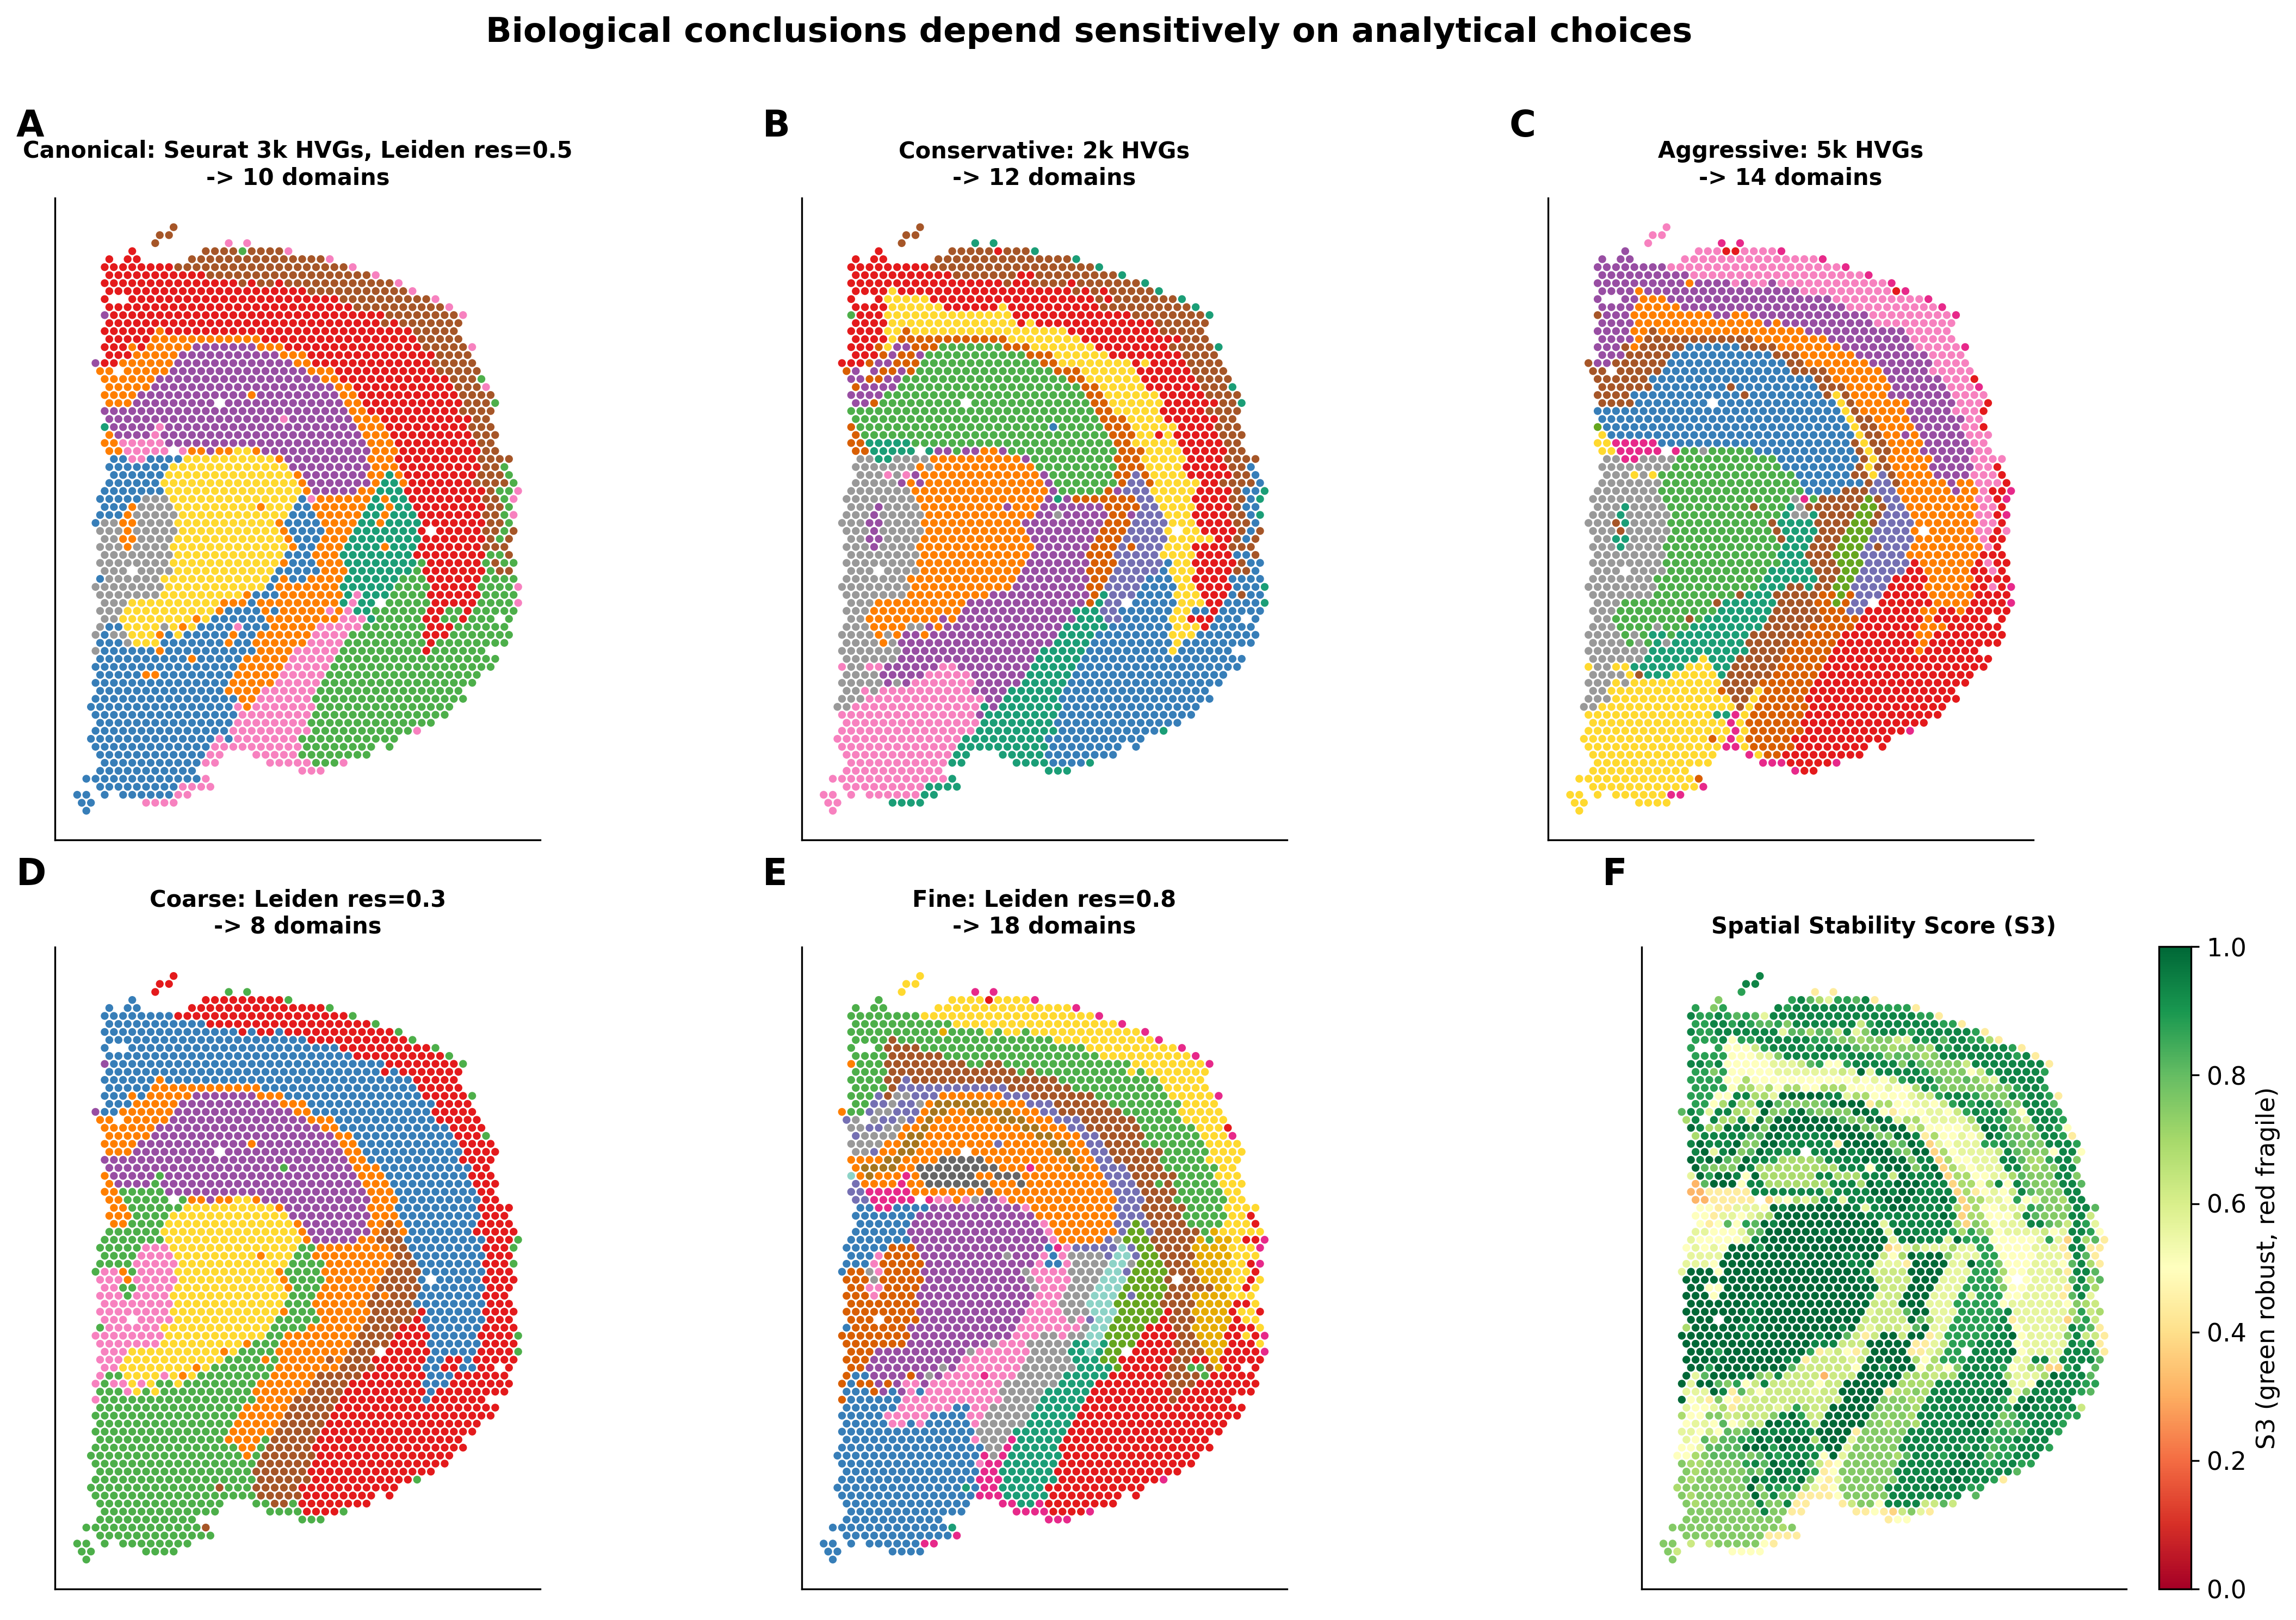
\includegraphics[width=\linewidth]{fig1_spec_montage.png}
  \caption{Mouse-brain H\&E section analyzed with five of the curated
  pipelines (A--E), which give 8--18 spatial domains. (F) Per-spot $S^3$
  across all \Nspecs{} curated pipelines (reference: canonical pipeline).}
  \label{fig:montage}
\end{figure}

\begin{figure}[t]
  \centering
  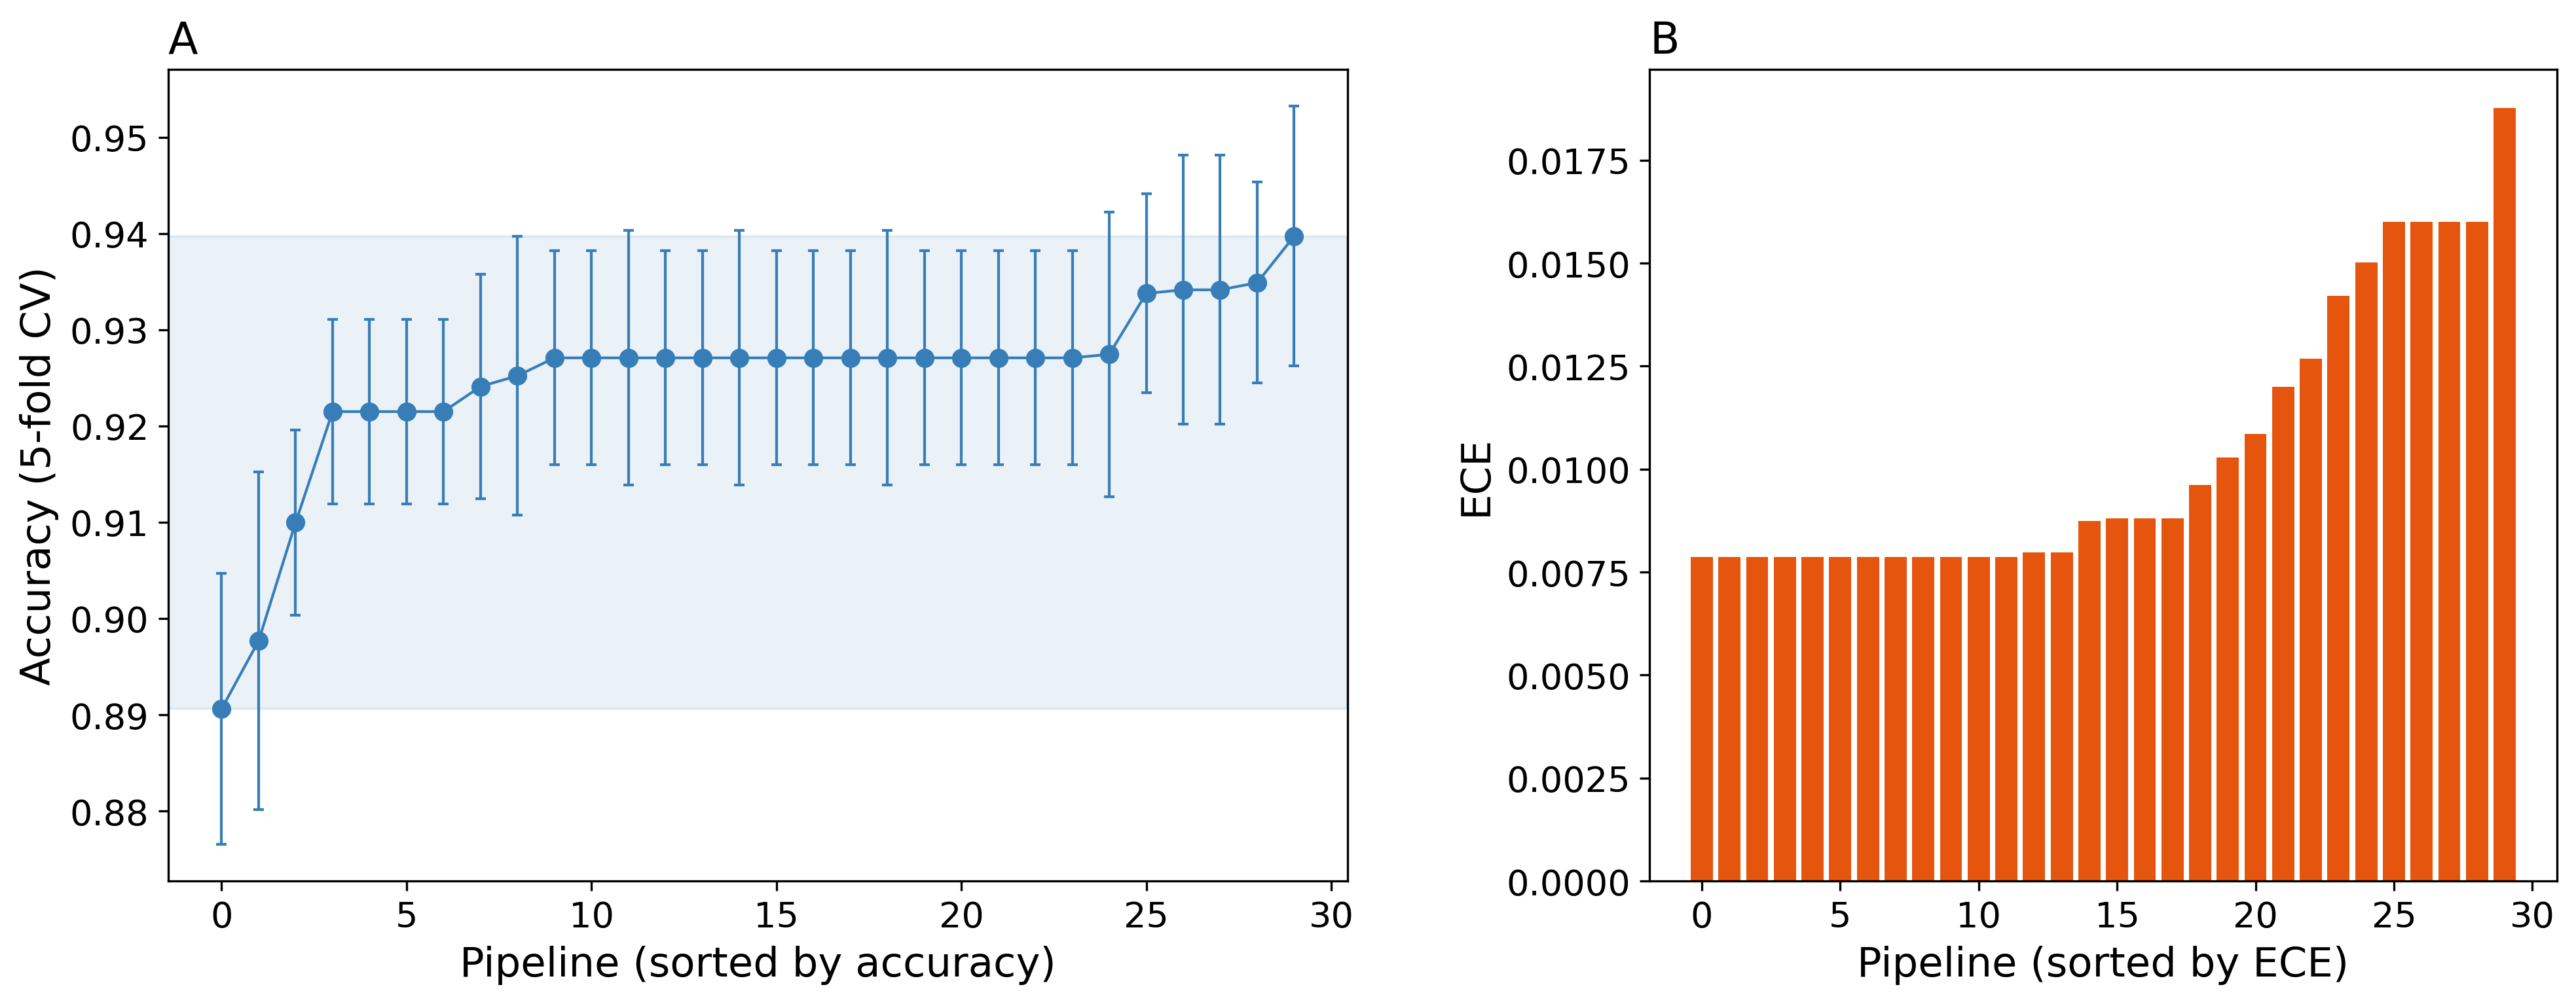
\includegraphics[width=0.9\linewidth]{12_downstream_ml.png}
  \caption{Accuracy and multiclass Brier score of a cross-validated
  anatomical-region classifier trained on each curated pipeline's embedding
  of the same mouse-brain section. Accuracy varies by \DownstreamRangePP{}
  percentage points across pipelines.}
  \label{fig:downstreamml}
\end{figure}

\begin{figure}[t]
  \centering
  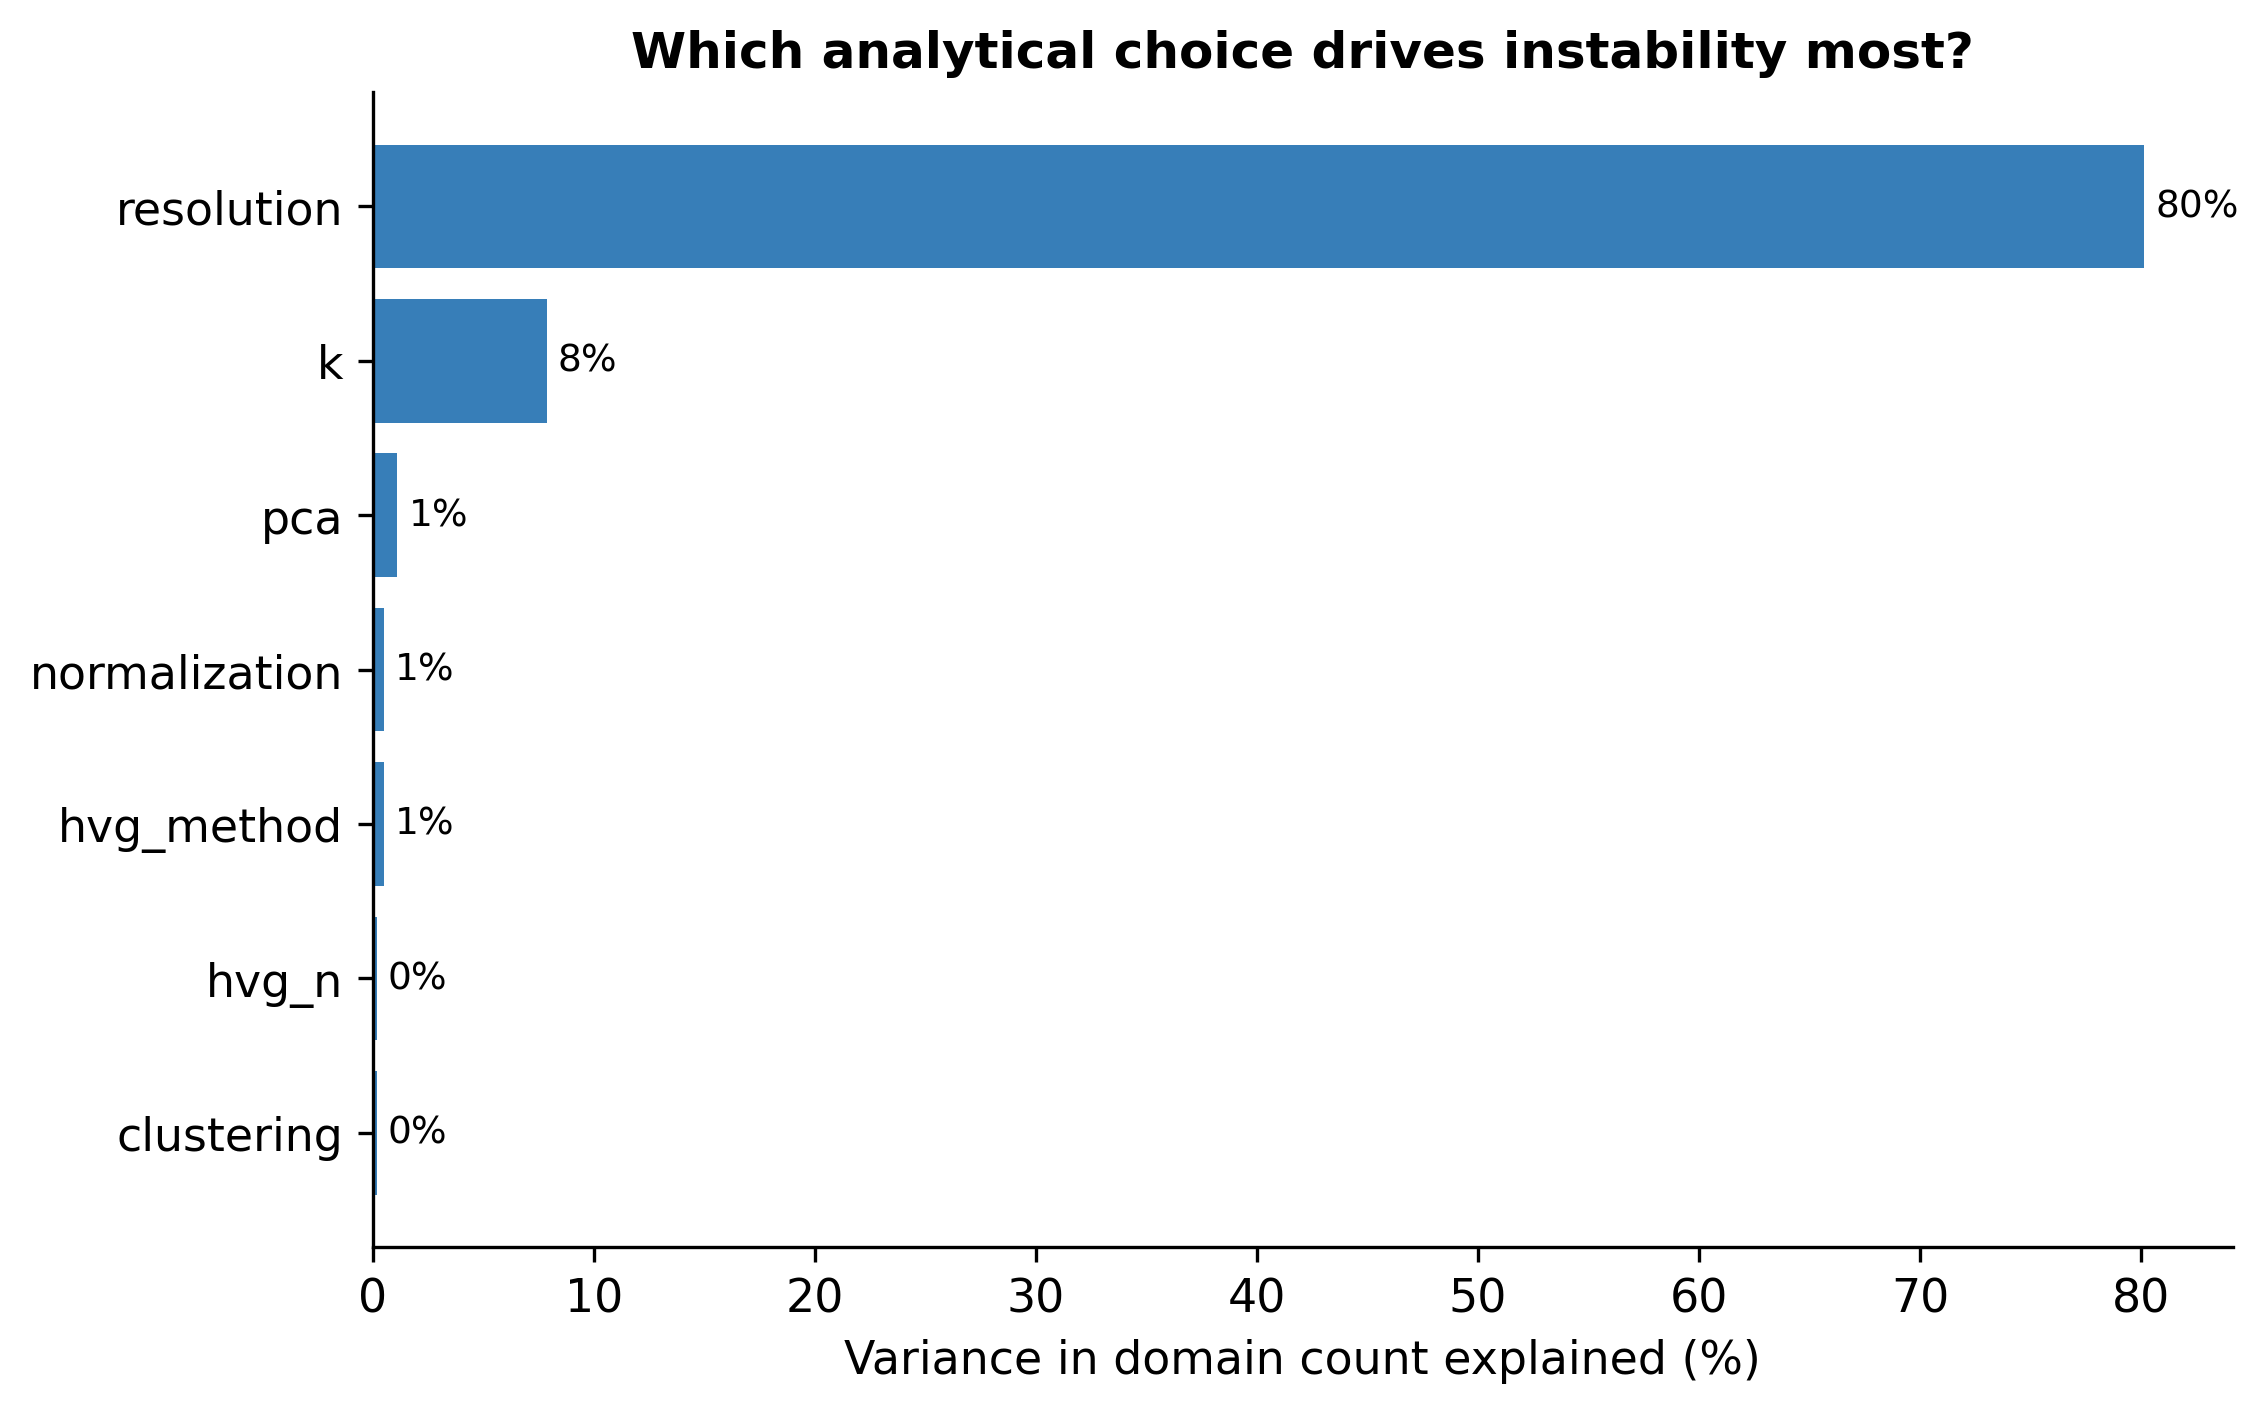
\includegraphics[width=0.85\linewidth]{08_variance_decomposition.png}
  \caption{Type-II ANOVA shares of variance in domain count for the curated
  mouse-brain pipelines (main effects only; axes correlated, so shares are
  approximate).}
  \label{fig:variance}
\end{figure}

\section{Results: Breast-Cancer Section}
\label{sec:tumor}

On the breast-cancer section with the curated pipelines, mean $S^3$ is
\TumorBoundaryS{} for boundary spots and \TumorInteriorS{} for interior
spots (gap \TumorGap{}; permutation $p\,\TumorStakesP{}$). Unlike in brain,
$S^3$ is correlated with sequencing depth ($r=\TumorConfoundR{}$ versus
$\ConfoundR{}$), and boundary spots have lower depth. The gap remains under
the depth-stratified test ($p\,\TumorDepthP{}$), with the caveats of
\S\ref{sec:stats}.

\textbf{Pathology annotations.} Using the SEDR annotations~\cite{fu2021sedr}
(Invasive, Tumor [in situ], Surrounding tumor, Healthy), mean $S^3$ is
\PathMarginS{} in the ``Surrounding tumor'' region, \PathInvasiveS{} in
the invasive region, and \PathHealthyS{} in healthy tissue (permutation
$p\,\PathP{}$; Fig.~\ref{fig:pathology}). The surrounding-tumor versus
invasive gap is \PathMarginInvasiveGap{} (95\% spot-bootstrap interval
$[\PathMarginInvasiveCILow{}, \PathMarginInvasiveCIHigh{}]$), and the
surrounding-tumor versus all-other-tissue gap is \PathMarginRestGap{}
($[\PathMarginRestCILow{}, \PathMarginRestCIHigh{}]$). These intervals
ignore spatial dependence and are likely too narrow. This is one section
from one patient, and ``Surrounding tumor'' is a dataset label, not a
verified surgical margin, so we make no general claim about tumor margins.

Resolution again has the largest share of variance in domain count
(\TumorVarTopFrac{}), followed by $k$ (\TumorVarKFrac{}) and normalization
(\TumorVarNormFrac{}). We had expected the dominant axis to differ from
brain; in this section it did not.

\begin{figure}[t]
  \centering
  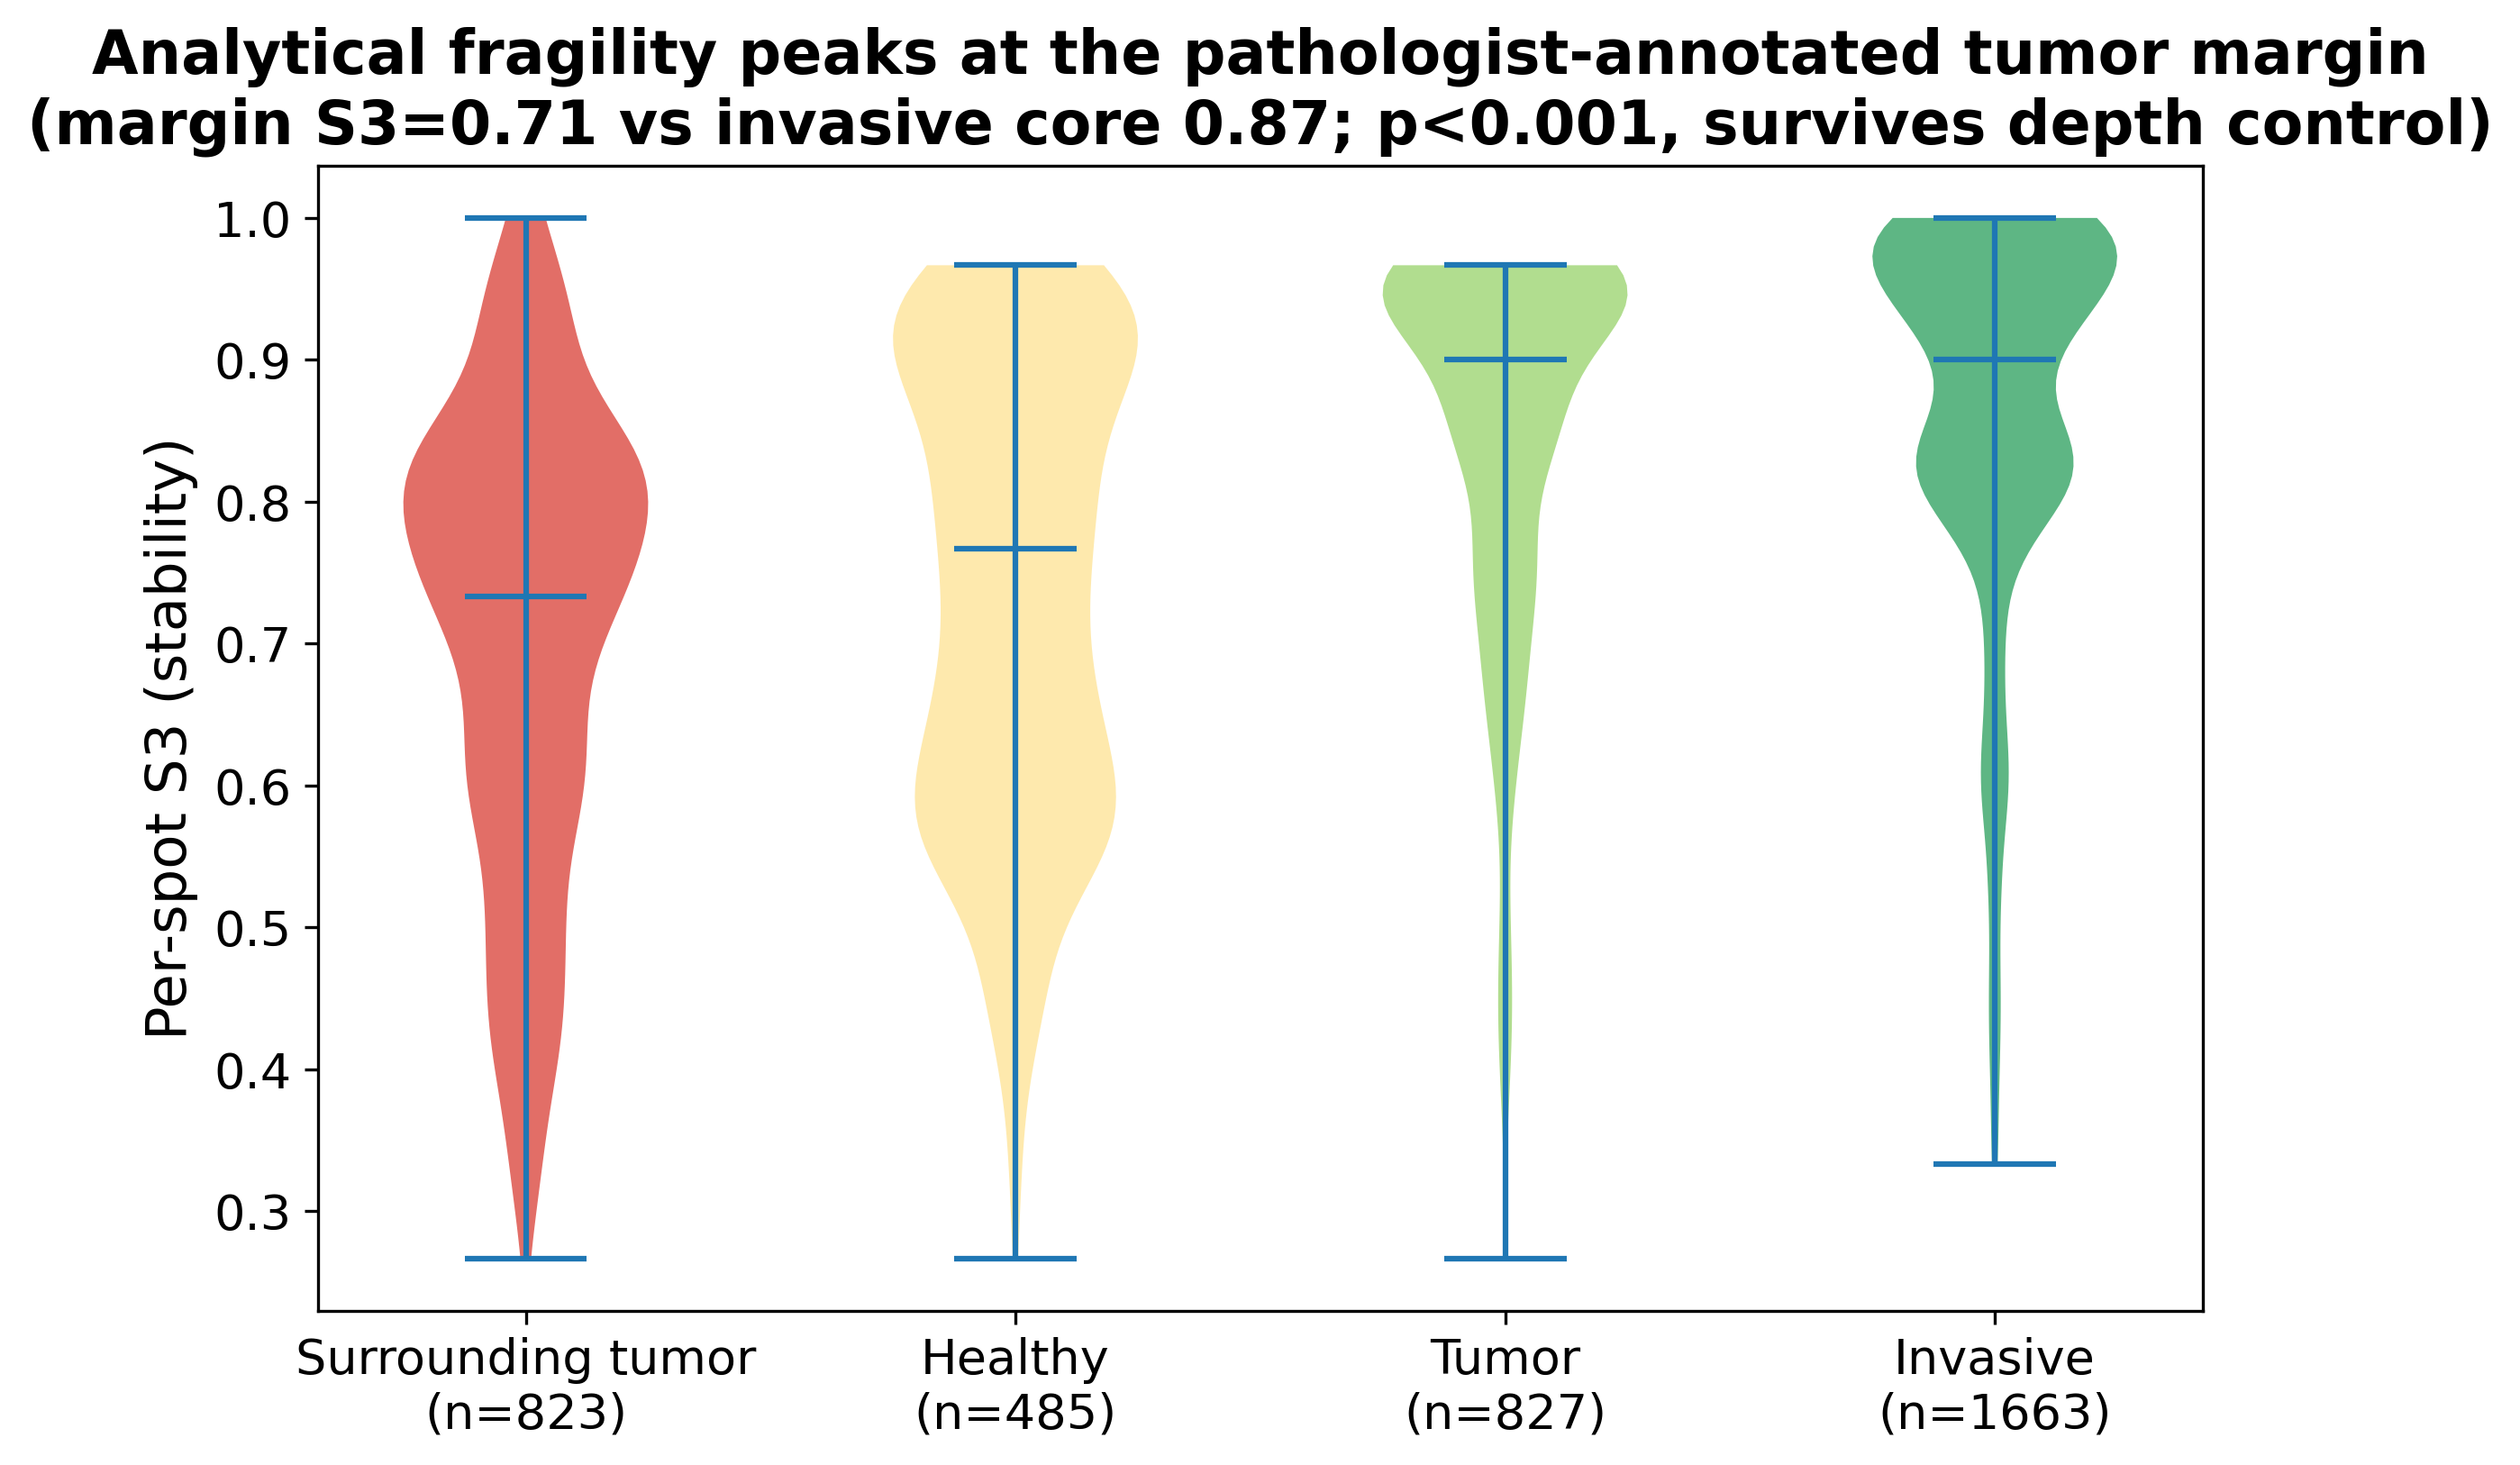
\includegraphics[width=0.9\linewidth]{16_pathology_stakes.png}
  \caption{Per-spot $S^3$ by SEDR pathology region on the breast-cancer
  section (curated pipelines). Annotations were made independently of all
  pipelines in this study.}
  \label{fig:pathology}
\end{figure}

\section{Full Factorial}
\label{sec:factorial}
We ran all \FullNspecs{} combinations in Table~\ref{tab:space} on the H\&E
mouse-brain section and the breast-cancer section. This design is balanced,
so the axes are uncorrelated and the Type-II shares approximately partition
the variance of the main-effects model; interactions remain in the
residual. Compared with the curated set, pipelines agree less (mean
pairwise ARI \FullAriHne{} vs.\ \AriMean{} in brain, \FullAriBreast{} in
tumor), and more spots have $S^3<0.5$ (\FullFragileHne{} in both sections).

Resolution again has the largest share (\FullVarResHne{} in brain,
\FullVarResBreast{} in tumor), followed by $k$ (\FullVarKHne{},
\FullVarKBreast{}). In tumor, HVG method (\FullVarHvgBreast{}) has a larger
share than normalization (\FullVarNormBreast{}), and the residual is
\FullResidBreast{} versus \FullResidHne{} in brain, which suggests larger
interactions between choices in that section. We did not fit interaction
terms or compute intervals for these shares. Boundary spots have lower
$S^3$ than interior spots in both sections (gap \FullGapHne{} in brain,
\FullGapBreast{} in tumor; permutation $p\,\FullGapP{}$ for both, with the
caveats of \S\ref{sec:stats}). We have not rerun the pathology, consensus,
or prediction analyses on the factorial.

\section{Exploratory: Consensus Across Pipelines}
\label{sec:consensus}

We build a co-association matrix (the fraction of curated specifications
that put each pair of spots in the same matched cluster) and cluster it
hierarchically to get consensus domains, on the mouse-brain H\&E section.
Single pipelines agree with the reference anatomy at ARI
\SingleWorstARI{}--\SingleBestARI{} (median \SingleMedianARI{}).

\textbf{Reference-informed upper bound.} We evaluated 18 consensus settings
(average or complete linkage, 10--18 clusters) against the reference. The
best reaches ARI \ConsensusARI{}, similar to the best single pipeline, and
\ConsensusBeatsMedianPct{} of the 18 settings exceed the median single
pipeline (Fig.~\ref{fig:consensus}). These settings are closely related, so
they are not independent comparisons, and choosing the best one uses the
reference.

\textbf{Reference-free selection.} Choosing the setting with the highest
mean silhouette width on the co-association distance, without the
reference, picks \ConsensusBlindLinkage{} linkage with
$k=\ConsensusBlindK{}$ (ARI \ConsensusBlindARI{}); across the grid,
silhouette and reference ARI have Spearman $\rho=\ConsensusSilARISpearman{}$.
This rule was checked only on the same section used to evaluate it, and we
have not compared the consensus with other ensemble methods.

Where the consensus disagrees with the reference, $S^3$ is lower (mean
$0.69$ vs.\ $0.81$), and $S^3$ separates correct from incorrect consensus
spots at ROC AUC \ConsensusUncAUC{} (consensus accuracy \ConsensusAcc{}).
Given the reference dependence of per-spot $S^3$ (\S\ref{sec:s3}), this is
exploratory.

\begin{figure}[t]
  \centering
  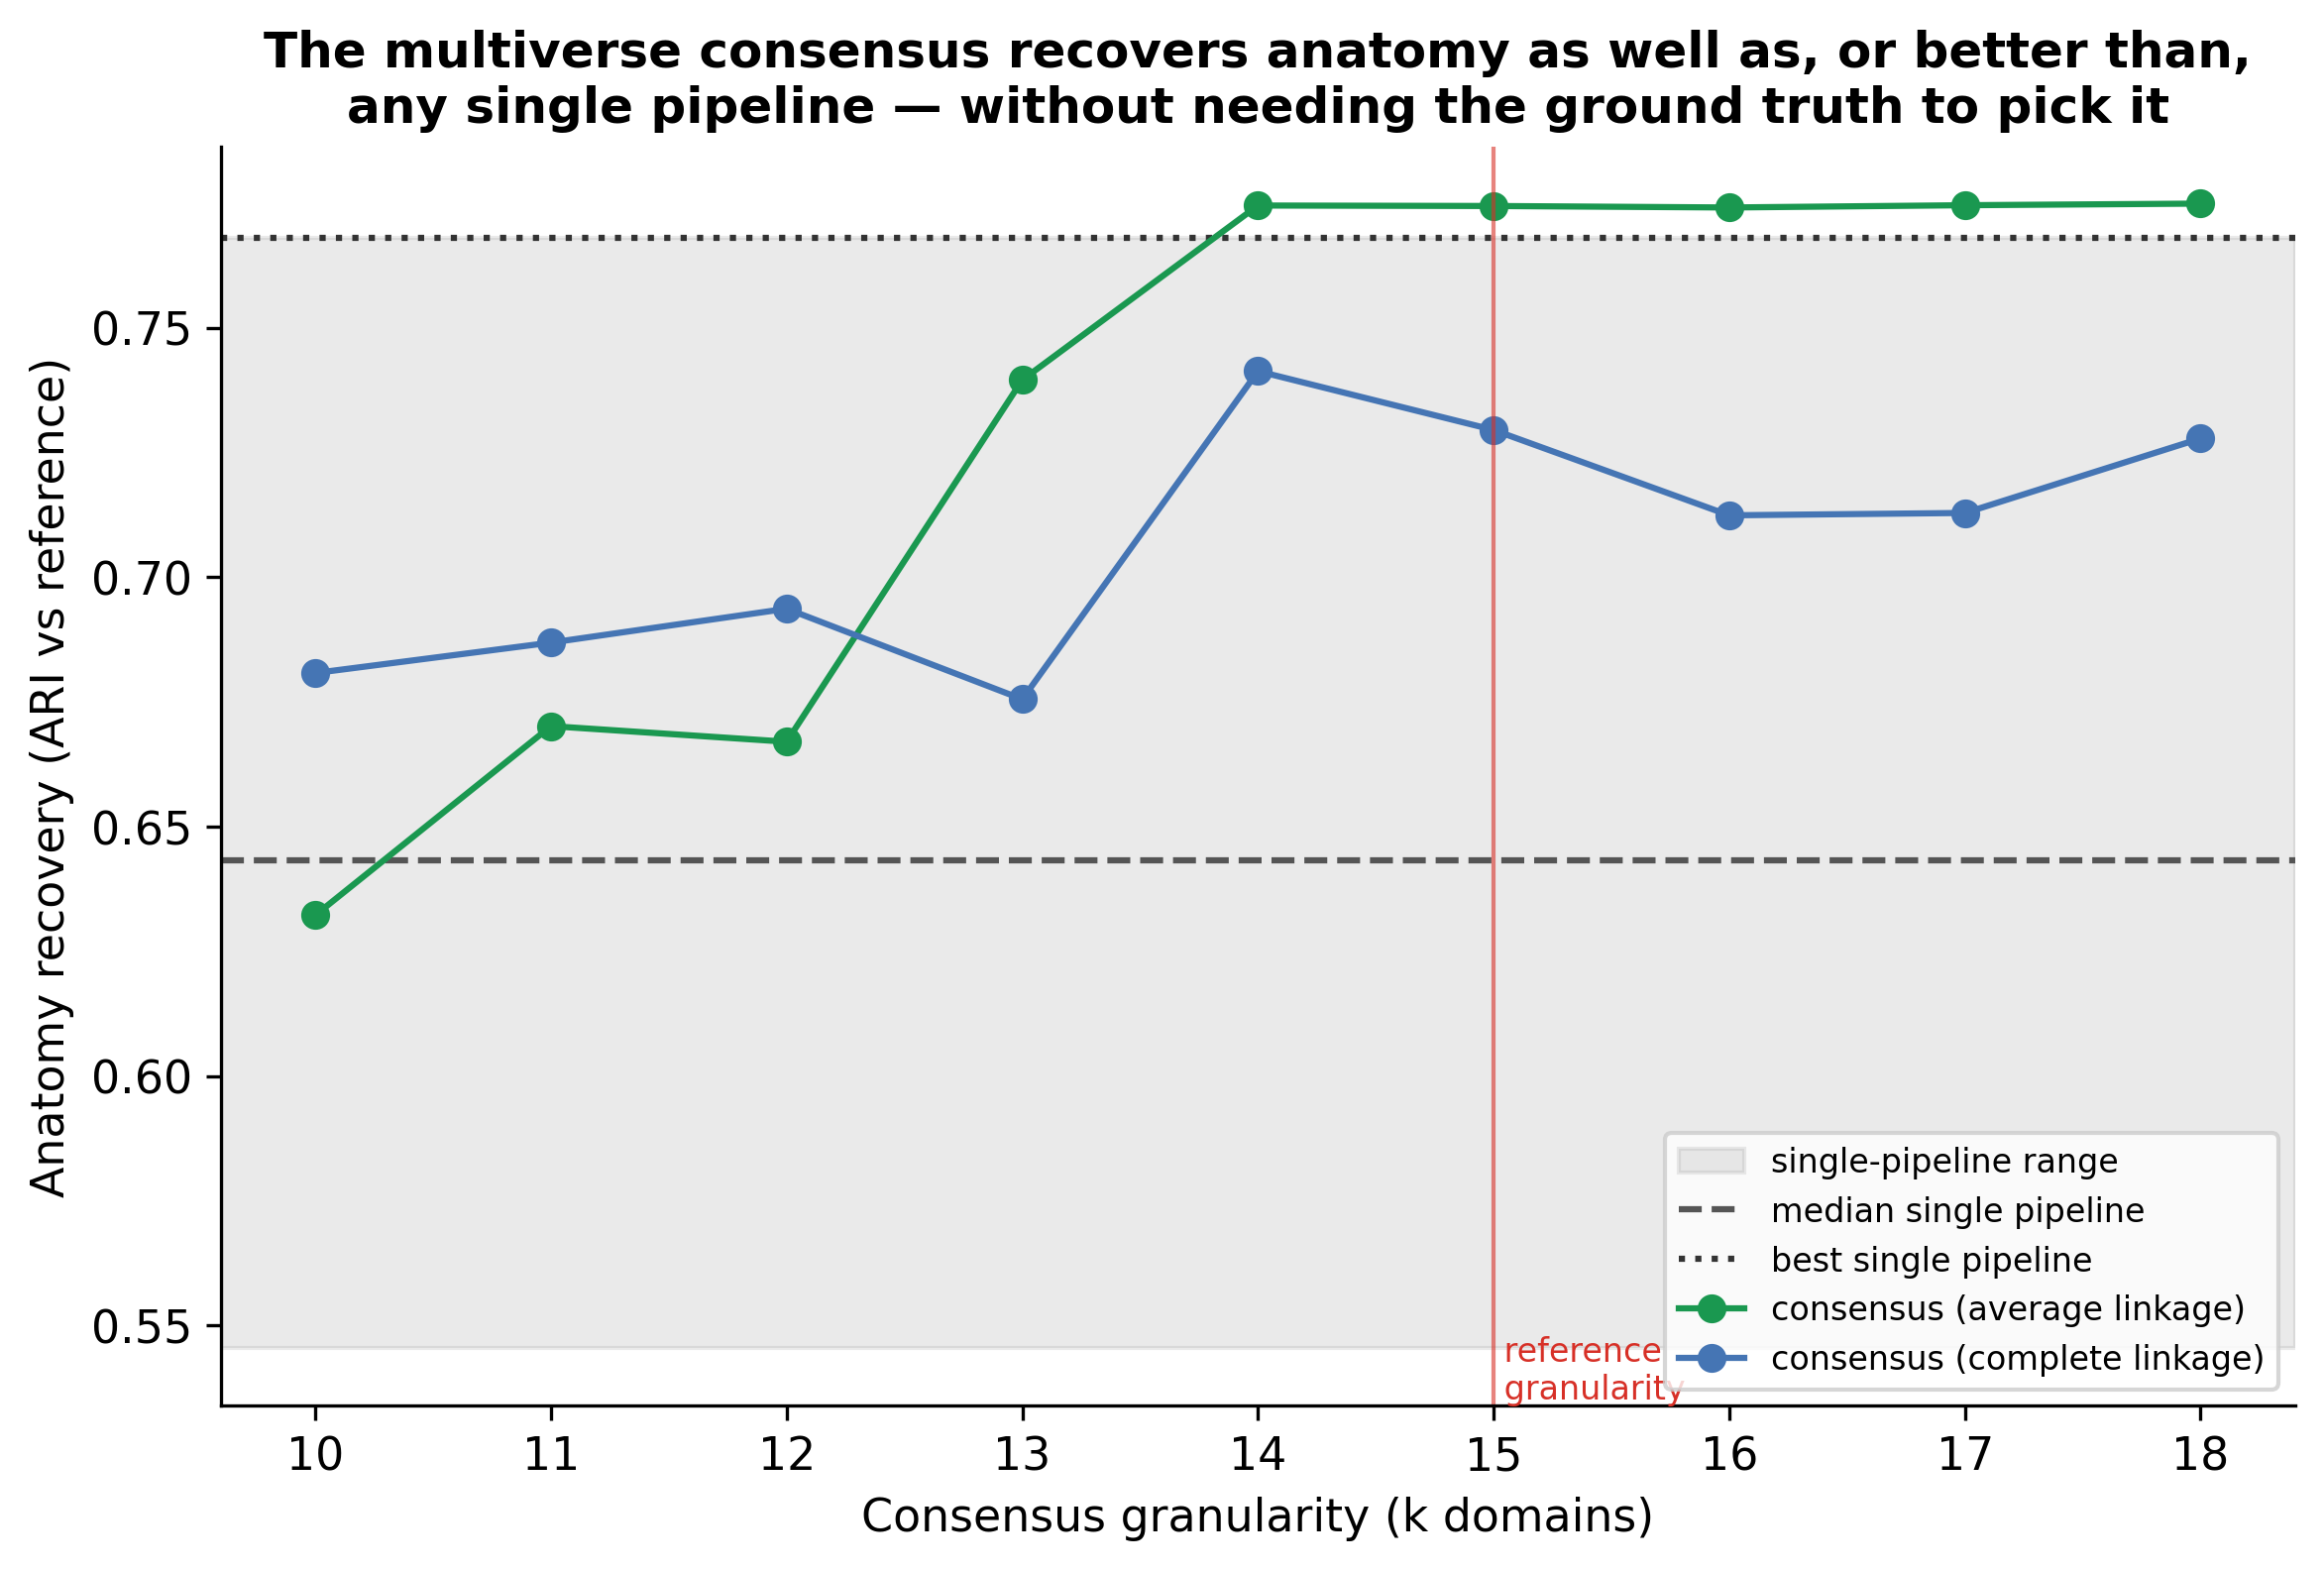
\includegraphics[width=0.9\linewidth]{15_consensus_recovery.png}
  \caption{ARI with the reference anatomy for 18 consensus settings
  (reference-informed upper bound) against the distribution of single
  curated pipelines, mouse-brain H\&E section.}
  \label{fig:consensus}
\end{figure}

\section{Exploratory: Predicting Low-Agreement Spots}
\label{sec:downstream}

We tested whether spots with $S^3<0.5$ in the curated set can be predicted
from features of one pipeline run on the mouse-brain H\&E section. The
target is this operational label, not biological unreliability. A logistic
regression uses four features from the canonical pipeline: local
transcriptomic heterogeneity (mean PCA distance to the 6 nearest spatial
neighbors), the fraction of those neighbors with a different cluster label,
total counts, and genes detected. With stratified 5-fold random
cross-validation, ROC AUC is \FragPredAUC{} (95\% bootstrap interval
$[\FragPredAUCRandomCILow{}, \FragPredAUCRandomCIHigh{}]$, label
permutation \FragPredPermP{}; Fig.~\ref{fig:fragpred}). Random splits put
neighboring spots in both training and test sets, so we also held out
\FragPredSpatialBlocks{} spatial blocks (k-means on coordinates) one at a
time (AUC \FragPredAUCSpatial{},
$[\FragPredAUCSpatialCILow{}, \FragPredAUCSpatialCIHigh{}]$) and then
removed training spots within \FragPredBufferMultiple{} median spot
spacings of the held-out block (\FragPredBufferDroppedPerFold{} spots per
fold on average; AUC \FragPredAUCBuffered{},
$[\FragPredAUCBufferedCILow{}, \FragPredAUCBufferedCIHigh{}]$). The best
single feature, neighbor disagreement, gives AUC $0.77$, and depth alone
gives $0.57$. All folds come from one section, so this does not show
transfer to new sections, specimens, or platforms.

\begin{figure}[t]
  \centering
  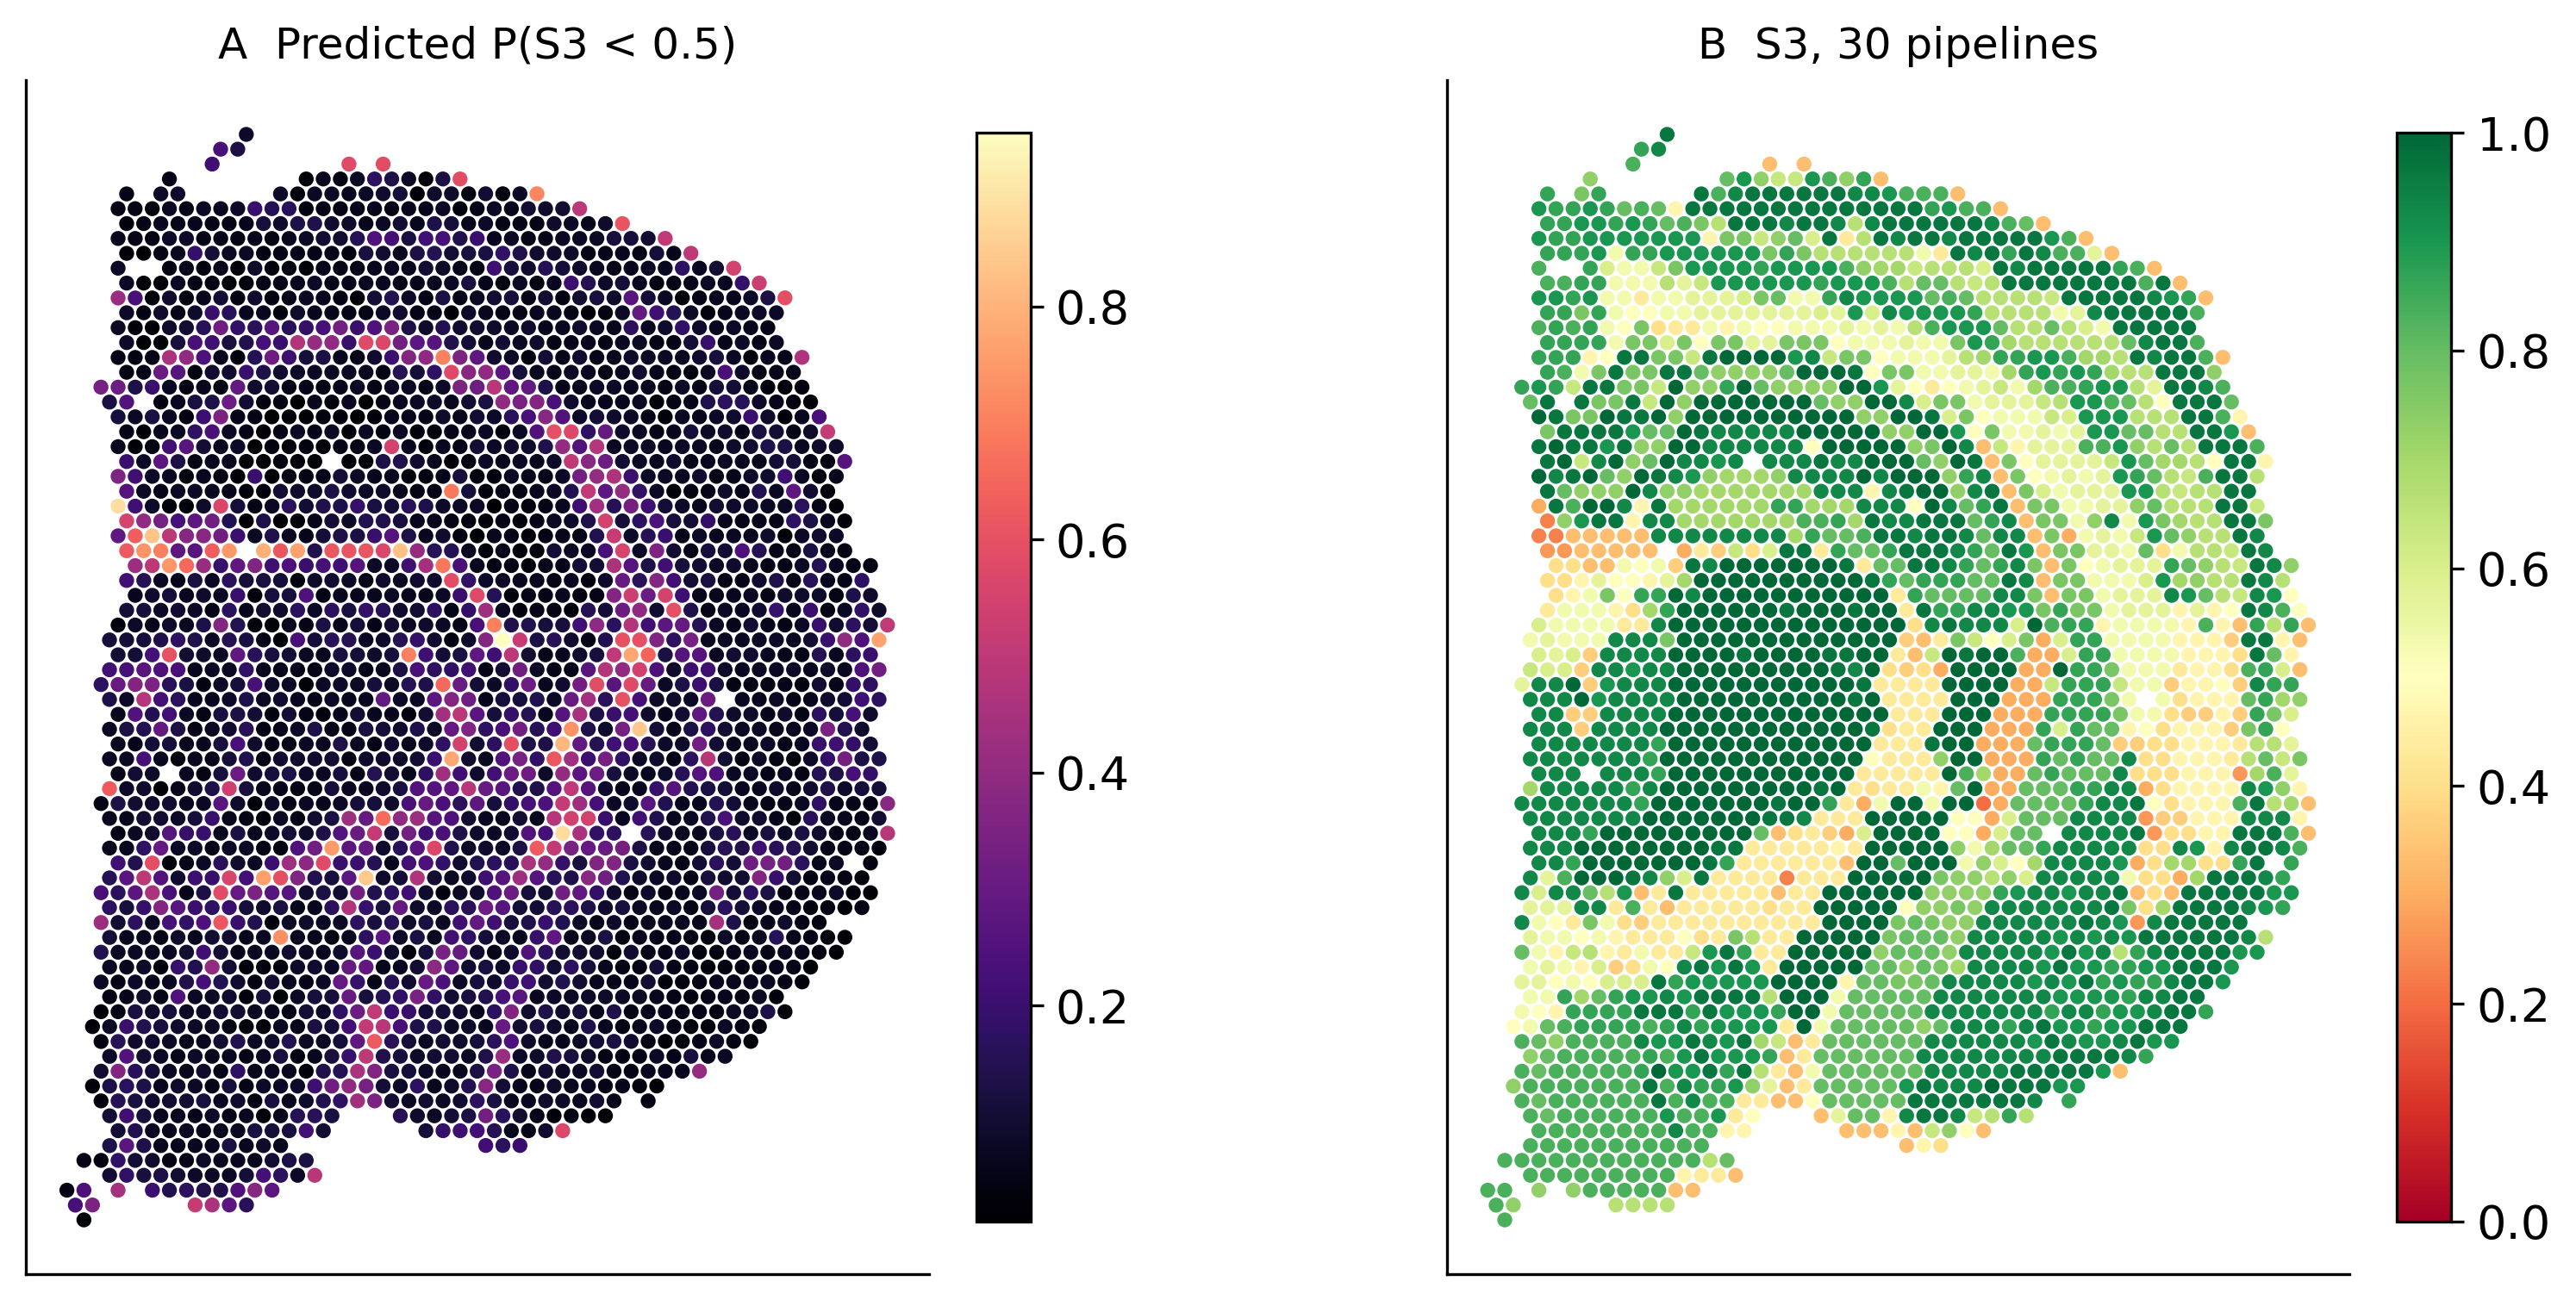
\includegraphics[width=0.9\linewidth]{17_fragility_prediction.png}
  \caption{Left: predicted probability that a spot has $S^3<0.5$, from one
  pipeline's local features (random split). Right: $S^3$ across the curated
  pipelines. Mouse-brain H\&E section.}
  \label{fig:fragpred}
\end{figure}

\section{Practical Notes}
In these sections, resolution changed the number of domains more than any
other setting, followed by $k$, both in the curated set and in the
factorial. Studies using similar pipelines should at least report both
values, and ideally show results at more than one resolution. SVG calls
near the significance threshold changed most across pipelines, so a
per-gene selection frequency is a useful addition to an SVG list. Whether
these patterns hold in other tissues and platforms is untested.

\section{Limitations}
This is a descriptive study of three sections: two mouse-brain sections of
unknown biological independence and one breast-cancer section from one
patient. Its results describe these sections and do not establish
generalization across animals, patients, tissues, or platforms. The
per-spot score depends on the reference pipeline and handles split and
merged clusters poorly (\S\ref{sec:s3}). The permutation tests and
bootstraps ignore spatial dependence, and we made no correction for
multiple comparisons. The variance shares come from a main-effects model
without intervals. The boundary proxy is derived from the pipelines and
was not varied in width. The SVG test was fixed. The consensus and
predictor were evaluated on the same section they were developed on. Next
steps are a label-free per-spot agreement measure, spatially blocked
permutations and bootstraps, factorial models with interactions, and more
sections with independent annotations.

\section{Conclusion}
Across 30 curated and 864 factorial pipelines on three public Visium
sections, reasonable analysis choices changed the number and extent of
spatial domains substantially, with clustering resolution and $k$
accounting for most of the variation in domain count. Agreement was lower
near label transitions in all three sections. These results argue for
reporting key settings and, where possible, results across several
pipelines.

\section*{Reproducibility}
Code, configuration, pinned package versions, aggregate tables, statistical
outputs, and figure scripts are at
\url{https://github.com/ImSpxrsh/MOSAIC-ISEF}. The \FullNspecs{}-pipeline
sweeps ran on the MIT ORCD Engaging cluster under Slurm, with 4 CPUs and
16 GB of memory per task and a median of about two minutes per pipeline.
Analyses use NumPy~\cite{harris2020array}, SciPy~\cite{virtanen2020scipy},
scikit-learn~\cite{pedregosa2011scikit}, SCANPY~\cite{wolf2018scanpy}, and
Squidpy~\cite{palla2022squidpy}.

\section*{Acknowledgments}
The authors acknowledge the MIT Office of Research Computing and Data for
providing high performance computing resources that have contributed to the
research results reported within this paper.

\section*{Use of AI Tools}
An AI assistant (Claude, Anthropic) was used to edit the prose of this
manuscript and to help write analysis code. All analyses, statistical
results, and claims were checked by the authors, who take full
responsibility for the content of this paper.


\bibliographystyle{IEEEtran}
\bibliography{references}

\end{document}
